\documentclass[10pt]{article}
\usepackage[margin=0.65in]{geometry}
\usepackage{amsmath,amssymb,amsthm,mathtools,enumitem,microtype,booktabs}
\usepackage{graphicx,multicol,caption}
\usepackage[compact]{titlesec}
\usepackage[hidelinks]{hyperref}
\usepackage[capitalise]{cleveref}
\titlespacing*{\section}{0pt}{4pt}{2pt}
\titlespacing*{\subsection}{0pt}{3pt}{1pt}
\setlist{nosep,leftmargin=*}
\setlength{\parskip}{2pt}\setlength{\parindent}{0pt}
\setlength{\tabcolsep}{4pt}

% ---------- theorem environments (shared counter) ----------
\theoremstyle{plain}
\newtheorem{theorem}{Theorem}
\newtheorem{lemma}[theorem]{Lemma}
\newtheorem{proposition}[theorem]{Proposition}
\newtheorem{corollary}[theorem]{Corollary}
\theoremstyle{definition}
\newtheorem{definition}[theorem]{Definition}
\newtheorem{assumption}{Assumption}
\renewcommand{\theassumption}{A\arabic{assumption}}
\theoremstyle{remark}
\newtheorem{remark}[theorem]{Remark}
\crefname{assumption}{Assumption}{Assumptions}
\crefname{proposition}{Proposition}{Propositions}

% ---------- macros ----------
\newcommand{\R}{\mathbb{R}}
\newcommand{\E}{\mathbb{E}}
\newcommand{\Hbar}{\bar H}
\newcommand{\epss}{\varepsilon_s}
\newcommand{\epsv}{\varepsilon_v}
\newcommand{\etaNL}{\eta_{\mathrm{NL}}}
\newcommand{\Ahat}{\hat A}
\newcommand{\Qhat}{\hat Q}
\newcommand{\Qstar}{Q^\star}
\newcommand{\Vstar}{V^\star}
\newcommand{\Dbar}{\bar\Delta}
\newcommand{\todo}[1]{\textbf{[TODO: #1]}}
\DeclareMathOperator{\val}{val}
\DeclareMathOperator{\expl}{expl}
\DeclareMathOperator{\TV}{TV}
\DeclareMathOperator{\Reg}{Reg}
\DeclareMathOperator{\range}{range}
\DeclareMathOperator{\lgs}{lgs}
\DeclareMathOperator{\gain}{gain}
\DeclareMathOperator*{\argmin}{arg\,min}
\DeclareMathOperator*{\argmax}{arg\,max}

\title{\vspace{-2.4em}\textbf{Per-Turn Equilibrium Play in Pok\'emon Random Battles:\\Error Budgets, Hedging over Experts, and Measured Exploitability}\vspace{-0.8em}}
\author{CS535 Final Project \quad [Name 1], [Name 2]}
\date{\vspace{-1.6em}}

\begin{document}
\maketitle

\begin{abstract}
\noindent
We study an agent for Gen~9 Pok\'emon Random Battles that solves a one-turn stage matrix with a heuristic leaf value by no-regret self-play (Regret Matching$^+$) every turn, solves one agent-form game over sampled opponent worlds (following PokaiTrainer \cite{Yu26}) under hidden information, and runs Hedge, an experts algorithm, over an MCTS expert and an equilibrium expert across games. Going beyond repeated play of one matrix game, we prove that its exploitability is at most $\Hbar(\epss+2\epsv+\text{sampling})$, where $\Hbar$ is the expected game length against a best response and the leaf error $\epsv$ does not shrink with compute. Empirically, time-matched MCTS with Foul Play's move rule beats equilibrium sampling (0.760 [0.677, 0.843]); a white-box exploiter gives 95\% lower bounds on exploitability of 0.250 for deterministic and 0.090 for sampled equilibrium play; carrying Hedge weights across games makes the learner harder to exploit (4 seeds; the CI just excludes 0; paired difference $+0.146$ [$+0.039$, $+0.253$]); and exact endgame solutions point to the leaf value as the bottleneck. RL best responses give no useful bound.
\end{abstract}

% =====================================================================
\section{Introduction}
\label{sec:intro}
In a Pok\'emon battle both players move simultaneously, damage, accuracy and critical hits are random, and, in Random Battles, each side's sets (moves, item, ability, Tera type) are drawn from a known generator and stay hidden until revealed: a zero-sum stochastic game with simultaneous moves and hidden information. The strongest public bot, Foul Play~\cite{foulplay}, instead samples opponent worlds and runs Monte Carlo tree search (MCTS) in each.

We study the equilibrium alternative. Each turn our agent enumerates both sides' legal actions, simulates one turn exactly over chance outcomes in the Rust engine poke-engine, scores each child position with a heuristic leaf value, and solves the resulting stage matrix with Regret Matching$^+$ (RM$^+$)~\cite{Tam14}. Under hidden information it samples opponent worlds and solves one agent-form game over them, following PokaiTrainer~\cite{Yu26}. Across games, Hedge~\cite{FS97,Gan15} mixes this equilibrium expert with an MCTS expert. This applies one principle, no-regret learning~\cite{Hannan57,LW94,FS97,CS535L6}, three times (\cref{sec:setting}): self-play inside a turn, an experts problem across turns and games, and, as a lens on MCTS, self-play without an adversarial guarantee. We ask how much exploitability per-turn equilibrium play can incur and which error dominates, how it compares with MCTS in strength and robustness, and whether a regret-minimising layer over both can stay strong and hard to exploit.

\textbf{Contributions.}
\begin{itemize}
\item \emph{From one matrix game to the whole battle: an error budget for per-turn solving} (\cref{sec:theory}, ours). This is our main step beyond the course's no-regret analysis, which treats repeated play of one known matrix~\cite{CS535L6}: we compose per-turn $\epss$-equilibria of \emph{estimated} stage matrices through a finite-horizon stochastic game with leaf error. Exploitability is at most $\Hbar$ times the per-turn solver, leaf and sampling errors, where $\Hbar$ is the game length against a best response; a counterexample shows that typical game length does not suffice, and the leaf term does not shrink with compute. The building blocks, backward induction~\cite{Shapley53}, the RM$^+$ regret bound and its alternating-update analysis~\cite{Tam14,BMS19}, and concentration~\cite{BLM13}, are prior work. We also give a hidden-information version with two further terms and show that both are needed.
\item \emph{The experts problem against an adaptive opponent, with stated guarantees} (\cref{sec:hedge}). Safety of Hedge relative to the surrogate matrix follows from the standard regret bound~\cite{FS97,HW98,CBL06}. The idea of no-regret selection between an equilibrium and an exploiting strategy is from Ganzfried and Sandholm \cite{Gan15}; our contribution is the finite-sample guarantee in the stochastic game and the carried-weights experiment. Ours are the regret constant for the anytime update as we implement it, the exact linear-regret rate of an incremental anytime update (extending a lower bound of~\cite{OP18}), which was a real bug in our first implementation, and a weight-dynamics identity that explains the experiment below (both in \cref{app:secondary}).
\item \emph{A head-to-head evaluation} (\cref{sec:exp}, ours). We compare equilibrium play with MCTS using Foul Play's move rule~\cite{foulplay} at matched time, the agent-form solve of~\cite{Yu26} with averaging over worlds, and Hedge with carried versus reset weights, all with 95\% confidence intervals.
\item \emph{Exploitability measurement} (\cref{sec:measure,sec:exp}). Valid lower bounds from fixed exploiters are textbook. Ours are a white-box search exploiter that certifies positive lower bounds for both equilibrium variants, and a negative result for RL best responses~\cite{Tim20}, which stay far from useful after a $68\times$ larger training budget.
\item \emph{Leaf diagnostics} (\cref{sec:leaf}, ours). Exact endgame solutions show that the leaf, not the solver, carries the error; one mis-scored terminal makes every affine calibration of the leaf constant; and a minimal non-termination example instantiates the Everett and Dubins--Savage phenomenon~\cite{Everett57,DS65,MS96}.
\end{itemize}
We make no Showdown ladder claims and no comparison with ladder bots such as Jaxcalibur~\cite{jaxcalibur}.

% =====================================================================
\section{Related work}
\label{sec:related}
\textbf{Pok\'emon agents.} Foul Play~\cite{foulplay} samples opponent sets and runs decoupled MCTS per sample in poke-engine, then samples among moves whose visit share is within 75\% of the top one. PokaiTrainer~\cite{Yu26} solves every VGC decision as a Bayesian matrix game under open team sheets; we use its agent-form formulation. Jaxcalibur~\cite{jaxcalibur} is a self-reported, closed-source ladder bot. Per-turn matrix solving with world sampling is therefore not new as a system; our contribution is the analysis and the measurement.

\textbf{Equilibrium computation and search.} Stage-wise backward induction for stochastic games goes back to Shapley~\cite{Shapley53}. Average no-regret self-play converges to equilibrium in zero-sum games~\cite{Hannan57,FS97,CBL06}, which underlies CFR and RM$^+$~\cite{Tam14,Tammelin15}; the alternating-update analysis of RM$^+$ is due to~\cite{BMS19}. Depth-limited re-solving (DeepStack, ReBeL, Student of Games~\cite{Mor17,Bro20,Sch23}) and CFR-D~\cite{CFRD} use leaves that depend on beliefs, which removes the non-locality error of determinized search~\cite{Fra98,Lon10} that our world-only leaves incur. Simultaneous-move MCTS converges approximately with Hannan-consistent selection~\cite{Lis13}. Our full-game bound has the shape of approximate dynamic programming error propagation~\cite{Mun07,Sch15,Per15}, made finite-horizon and adversarial.

\textbf{Regret, RL and exploitability.} No external regret goes back to Hannan~\cite{Hannan57} and weighted majority to Littlestone and Warmuth~\cite{LW94}; Hedge, fixed share and anytime tuning are standard~\cite{FS97,HW98,CBL06}. Policy optimisation is online learning per state: natural policy gradient is Hedge on $Q$-values~\cite{Aga21}, and TRPO/PPO-style updates are mirror descent~\cite{Tom22,Sha20}; see also~\cite{Pol19,Ross11}. Policy-gradient methods reach last-iterate convergence in games through regularisation~\cite{Sok23,Per22} and are reported competitive with CFR-style deep RL~\cite{Rud25}. Our guarantee on exploiting opponents is external regret only; stronger comparators are statistically hard in Markov games~\cite{Tian21,Liu22}, and policy regret against adaptive adversaries is unattainable in general~\cite{Aro12b}. Exploitability is estimated from below by RL best responses~\cite{Tim20,Lan17}, which can defeat frozen superhuman agents~\cite{Wang23}, or by local search~\cite{Lis17}. Our surrogate-to-true transfer term plays the role of the model error in the simulation lemma~\cite{KS02}.

% =====================================================================
\section{Preliminaries: no-regret learning and games}
\label{sec:prelim}
\textbf{The experts problem and external regret} (notation of~\cite{CS535L6}). There are $n$ experts and $T$ rounds. In round $t$ Nature fixes losses $l^t_i\in[0,1]$; without seeing them, the algorithm chooses a distribution $p^t$ over the experts and follows an expert drawn from it; then all losses are revealed. \emph{Adversary model:} Nature may depend on everything that happened earlier and may know the algorithm, hence $p^t$, but not the current random draw. The (external) regret is the expected total loss minus that of the best fixed expert in hindsight, $\Reg_T=\sum_tp^t\cdot l^t-\min_i\sum_tl^t_i$, and an algorithm is \emph{no-regret} if $\Reg_T=o(T)$~\cite{Hannan57}. Every deterministic map from past losses to an expert suffers linear regret, because Nature can predict its choice and give that expert loss 1 (follow-the-leader is the standard example), so beating an adversary requires randomisation.

\textbf{Multiplicative weights.} MWU (randomised weighted majority~\cite{LW94}, Hedge~\cite{FS97}) starts from $w^1_i=1$, plays $p^t_i=w^t_i/\sum_jw^t_j$ and updates $w^{t+1}_i=w^t_i(1-\eta l^t_i)$ with $\eta\in(0,\frac12]$. A potential argument on $\sum_iw^t_i$ gives $L_{\rm MWU}\le(1+\eta)L^*+\ln n/\eta$, where $L^*$ is the best expert's total loss; for $T\ge4\ln n$ and $\eta=\sqrt{\ln n/T}$ this is $\Reg_T\le2\sqrt{T\ln n}$.

\textbf{No-regret self-play.} Let $A\in[0,1]^{n\times m}$ pay the row player (Row, maximiser) and cost the column player (Column), with $v_R=\max_x\min_yx^\top Ay$ and $v_C=\min_y\max_xx^\top Ay$. Both players run a no-regret algorithm on the repeated game with full-information feedback: Row's loss for row $i$ is $1-e_i^\top Ay^t$ and Column's loss for column $j$ is $(x^t)^\top Ae_j$. Let $\bar x,\bar y$ be the average strategies, $\bar g=\frac1T\sum_t(x^t)^\top Ay^t$ Row's average payoff, and $\epsilon_R,\epsilon_C$ the two average regrets.
\begin{proposition}[no-regret self-play~\cite{FS97,CS535L6}]\label{prop:selfplay}
$v_C-\epsilon_R\le\bar g\le v_R+\epsilon_C$ and $\max_xx^\top A\bar y-\min_y\bar x^\top Ay\le\epsilon_R+\epsilon_C$. Hence $(\bar x,\bar y)$ is an $(\epsilon_R+\epsilon_C)$-approximate minimax equilibrium, and $\min_y\bar x^\top Ay\ge\val(A)-\epsilon_R-\epsilon_C$.
\end{proposition}
\emph{Proof idea.} By Row's regret and linearity, $\bar g\ge\max_i\frac1T\sum_te_i^\top Ay^t-\epsilon_R=\max_xx^\top A\bar y-\epsilon_R\ge v_C-\epsilon_R$; symmetrically $\bar g\le\min_y\bar x^\top Ay+\epsilon_C\le v_R+\epsilon_C$; rearrange. The proof uses only the two regret inequalities and linearity, so it holds for any no-regret learners, for weighted averages with weighted regrets, and for a matrix of range $\Delta$ after rescaling. In general-sum games the same argument yields a coarse correlated equilibrium (CCE); our game is two-player zero-sum, where the marginals of a CCE are minimax strategies, so we do not need CCE.

% =====================================================================
\section{Method: one principle, three applications}
\label{sec:setting}
\textbf{Game.} We model a battle as a finite-horizon, two-player, zero-sum stochastic game with finite states, horizon $H$ (the 300-turn cap), simultaneous actions $a\in A(s)$ and $b\in B(s)$, chance transitions $P(\cdot\mid s,a,b)$, and terminal payoffs $u\in\{-1,0,1\}$ (loss, draw or cap, win). With $\val(A)=\max_x\min_y x^\top Ay$, the true stage matrix and value are $\Qstar_t(s)(a,b)=\sum_{s'}P(s'\mid s,a,b)\Vstar_{t+1}(s')$ and $\Vstar_t(s)=\val\Qstar_t(s)$; every stage matrix has range $\Delta\le2$. The agent $\pi$ is the row player, and its exploitability is $\expl(\pi)=\Vstar_0(s_0)-\inf_\sigma W^{\pi,\sigma}_0(s_0)$, where $W$ is the expected payoff and the opponent $\sigma$ may condition on the whole history. We report scores $s=(u+1)/2\in[0,1]$ (wins plus half of draws); in score units exploitability is halved and the symmetrised game has value $v^\star=\frac12$. We write $n,m\le13$ for the numbers of legal actions and $\tau\le H$ for the stopping turn.

\subsection{Inside a turn: no-regret self-play}
\label{sec:inside}
\textbf{Stage matrix and solver.} At $(t,s)$ the agent builds an estimate $\Qhat_t(s)$: an unpruned depth-2 expectiminimax matrix whose cells average a leaf value over all chance outcomes of one simulated turn. The leaf is the midpoint of the two sides' maximin values from the engine's depth-1 search, in heuristic engine units. The agent runs $T$ iterations of the no-regret algorithm RM$^+$ for both sides on $\Qhat_t(s)$, which is the self-play of \cref{prop:selfplay} with full-information feedback, and then plays the averaged strategy (\emph{equilibrium, sampled}), its most probable action (\emph{equilibrium, top move}), or the pure maximin row (\emph{safest move}). We write $\epss$ for the solver's gap in $\Qhat$ and $\epsv=\lVert\Qhat_t(s)-\Qstar_t(s)\rVert_\infty$ for the leaf error.

\textbf{Deviation from the lectures.} We use alternating updates (Column's iterate responds to Row's new one, rather than both moving from the same history) and linear averaging, $\bar x=\sum_tt\,x_t/\sum_tt$, not the uniform average. \Cref{prop:selfplay} goes through with $t$-weighted regrets; alternation adds the cross term $\sum_tt\,[u(x_t,y_t)-u(x_t,y_{t-1})]$, which is $\le0$ for RM$^+$ (\cite{BMS19}, Thm~5). With the RM$^+$ regret bound~\cite{Tam14} this gives the stage solution's quality:
\begin{proposition}[solver rate]\label{prop:rm}
RM$^+$ with alternating updates and linear averaging gives $\epss\le2\Delta(\sqrt n+\sqrt m)/\sqrt T$, which is at most $8\sqrt{n/T}$ for $\Delta=2$ and $m\le n$.
\end{proposition}

\textbf{Hidden information.} Each side sees its own team and what the opponent has revealed. The belief $b$ is the exact posterior over each revealed Pok\'emon's sets given the revealed moves and Tera type. The agent samples $K=4$ worlds with stage matrices $M_k$ and solves the agent-form game $\max_x\sum_k b_k\min_j(M_k^\top x)_j$ as one linear program, so the opponent best-responds in each world~\cite{Yu26}. The baseline \emph{PIMC blend} averages the per-world equilibria instead.

\subsection{Across turns and games: the experts problem against an adaptive opponent}
\label{sec:hedge}
Equilibrium play is safe but leaves value on the table, while MCTS is strong but exploitable (\cref{sec:exp}). This is the lectures' rock-paper-scissors ``hustler''~\cite{CS535L6}: exploit the opponent's flaws, but retreat to the safe equilibrium when it plays well, i.e.\ safe opponent exploitation~\cite{Gan15}. We cast it as the experts problem of \cref{sec:prelim} with the real opponent as Nature. The learner keeps weights $w_t$ over $k$ experts with stage strategies $q_{e,t}$ and plays $p_t=\sum_e w_{t,e}q_{e,t}$. After the opponent's move $b_t$ it rewards every expert counterfactually under the heuristic matrix $\Ahat_t$,
$r_{t,e}=\mathrm{clip}\big((q_{e,t}\cdot\Ahat_t[:,b_t]-\min\Ahat_t)/\Dbar,0,1\big)$ with a fixed normaliser $\Dbar=400$ engine units. The update is anytime FTRL, $\log w_t=\eta_{t-1}L_{t-1}$ with $L_t=\sum_{j\le t}r_j$ and $\eta_t=\sqrt{8\ln k/t}$. We use $k=2$ experts, $F$ (MCTS with Foul Play's move rule) and $N$ (equilibrium, sampled), and let $t$ count non-forced turns. The weights are either reset at the start of each game or carried across the games of a match.

\textbf{Relation to the lectures.} Rewards are normalised to $[0,1]$, as the experts problem requires; the loss is $l=1-r$, and $\Reg_T=\max_e\sum_{t\le T}r_{t,e}-\sum_{t\le T}w_t\cdot r_t$ is external regret with $k$ experts. Our update is the exponential-weights form with a decreasing step, not $w\leftarrow w(1-\eta l)$ with $\eta$ tuned to a known $T$; both give regret of order $\sqrt{T\ln k}$, with constant 2 for MWU and $\frac32/\sqrt2$ for ours (\cref{lem:R2}). Three departures: the experts recommend stage strategies that change every turn and we play their mixture rather than one sampled expert, so the bound holds on every path rather than in expectation; rewards are counterfactual payoffs in the surrogate $\Ahat_t$, not game outcomes; and the opponent, which may know $p_t$ but not our sampled action, as in the lectures' adversary model, also changes which states we visit, so the comparator is the best expert along our own trajectory (external, not policy, regret~\cite{Aro12b}). Carried weights make a match one long experts problem ($T$ = all non-forced turns of the match); reset weights start a short one each game ($T\approx$ one game's length), so only the carried learner's regret bound per turn keeps shrinking.

\begin{assumption}[equilibrium expert]\label{asm:E} At every learner turn one expert ($N$) is an $\epss$-equilibrium strategy of $\Ahat_t$.\end{assumption}

\begin{lemma}[anytime FTRL as implemented]\label{lem:R2}
With step sizes $\beta_1\ge\beta_2\ge\dots>0$ and $w_t\propto\exp(\beta_tL_{t-1})$, for adaptively chosen rewards in $[0,1]^k$, $\Reg_T\le\ln k/\beta_T+\frac18\sum_t\beta_t$ on every path. For $\beta_t=\eta_{t-1}$, $\Reg_T\le\tfrac32\sqrt{T\ln k/2}+\sqrt{\ln k/8}$.
\end{lemma}
The textbook bound (\cite{CBL06}, Thm~2.3) uses $\eta_t$ at turn $t$; the constant above is proved for our indexing.

\begin{proposition}[safety relative to the surrogate]\label{prop:E1}
Under \cref{asm:E}, on every path and against any adaptive opponent, $\sum_{t\le S}p_t\cdot\Ahat_t[:,b_t]\ge\sum_{t\le S}(\val\Ahat_t-\epss)-\Dbar\Reg_S$ over $S$ learner turns.
\end{proposition}
The guarantee is relative to $\Ahat_t$, not to win probability, and it requires the fixed normaliser (\cref{app:proofs}). Symmetrically, the learner's surrogate payoff is at least the best expert's minus $\Dbar\Reg_S$ (the hustler's exploitation side), but this is external regret along the learner's own trajectory, not policy regret~\cite{Aro12b}. With \cref{thm:full}, \cref{prop:E1} bounds the average per-game loss of carried weights if one global affine map $a\Ahat+c$ with $a>0$ approximates $\Qstar$ (\cref{app:proofs}); our leaf violates this (\cref{sec:leaf}). \Cref{app:secondary} shows that the incremental anytime update of our first implementation has linear regret (\cref{prop:R1}) and gives the weight dynamics (\cref{lem:R3}).

\subsection{Inside MCTS: the same self-play view}
\label{sec:mcts}
At a node of decoupled MCTS each side runs the bandit algorithm UCB1 on the node's matrix, and the visit shares are its average strategies: self-play with bandit rather than full-information feedback. With exact regrets, \cref{prop:selfplay} holds with equality.
\begin{proposition}[visit shares]\label{prop:visits}
At one node let side one maximise $\Ahat\in[0,1]^{n\times m}$ and side two $1-\Ahat$, with returns of conditional mean $\Ahat(a_i,b_i)$. With visit shares $\bar x_N,\bar y_N$ and mean-reward external regrets $\Reg^1_N,\Reg^2_N$ after $N$ simulations, $\max_a(\Ahat\bar y_N)_a-\min_b(\bar x_N^\top\Ahat)_b=(\Reg^1_N+\Reg^2_N)/N$.
\end{proposition}
Visit shares and RM$^+$ averages are thus the same object~\cite{Lis13}, and the shares converge exactly when the summed regret is sublinear. UCB1 is designed for stochastic bandits and has no guarantee against an adaptive opponent, which the other side's learner is, so the hypothesis of \cref{prop:selfplay} is not supplied, and the shares can fail to converge even on a $2\times2$ matrix with a dominant row (\cref{app:proofs}).

% =====================================================================
\section{Theory: from one matrix game to the whole battle}
\label{sec:theory}
\Cref{prop:selfplay} concerns repeated play of \emph{one} known matrix game. In a battle every turn has a new stage matrix, that matrix is only an estimate built from a heuristic leaf, and the turns are linked through a finite-horizon stochastic game whose length the opponent can influence. Our main step beyond the lectures is to compose per-turn $\epss$-equilibria of the estimated matrices through this game, charging the leaf error explicitly. The main bound uses three assumptions. Without the first two, two further per-turn terms appear, a non-locality gap and a belief error, and both are necessary (\cref{thm:C} in \cref{sec:general}).
\begin{assumption}[non-revealing opponent]\label{asm:nonrev} The opponent's actions do not depend on its hidden sets, so behavioural evidence does not move the true posterior away from our belief. This holds trivially under full information.\end{assumption}
\begin{assumption}[world-only leaves]\label{asm:world} The value after the lookahead depends on the true position, not on what each side believes; concealment then has no value.\end{assumption}
\begin{assumption}[exact prior]\label{asm:prior} Opponent sets are drawn from the Random Battle generator, and the agent samples from that generator.\end{assumption}

\begin{lemma}[one turn]\label{lem:one}
Let $\lVert A-B\rVert_\infty\le\varepsilon$ and let $x$ be $\epss$-optimal in $B$. Then $\min_y x^\top Ay\ge\val(A)-\epss-2\varepsilon$, and the factor $2$ is tight.
\end{lemma}

\begin{theorem}[whole game, full information]\label{thm:full}
Let the agent be Markov, with $\lVert\Qhat_t(s)-\Qstar_t(s)\rVert_\infty\le\epsv$ and $\epss$-optimal stage play in $\Qhat_t(s)$, and put $\delta=\epss+2\epsv$. For every history-dependent opponent $\sigma$, $W^{\pi,\sigma}_0(s_0)\ge\Vstar_0(s_0)-\E_{\pi,\sigma}\big[\sum_{t<\tau}\delta(t,s_t)\big]$. Hence, for a best response $\sigma^\star$ with $\Hbar=\E_{\pi,\sigma^\star}[\tau]$,
\begin{equation}\label{eq:full}
\expl(\pi)\;\le\;\Hbar\,(\epss+2\epsv)\;\le\;H(\epss+2\epsv).
\end{equation}
\end{theorem}
\emph{Proof sketch.} Backward induction over histories shows $W_t(h)\ge\Vstar_t(s_t)-D_t(h)$, with $D_t$ the conditional expected sum of remaining budgets; each step applies \cref{lem:one} at the opponent's actual stage mixture (\cref{app:proofs}).

The factor $\Hbar$ cannot be replaced by the typical game length: in a chain where a minimax-optimal opponent ends the game at once, an opponent that always continues extracts $H\delta$, so \eqref{eq:full} holds with equality (\cref{app:proofs}).


\begin{corollary}[error budget]\label{cor:headline}
Under \cref{asm:nonrev,asm:world,asm:prior}, with \cref{prop:rm} and the sampling bound of \cref{prop:K} (\cref{sec:general}),
\begin{equation}\label{eq:headline}
\expl(\pi)\;\le\;\Hbar\Big(\underbrace{8\sqrt{n/T}}_{\text{solver}}+\underbrace{2\epsv}_{\text{leaf}}+\underbrace{4\sqrt{2n\log K/K}}_{\text{sampled worlds}}\Big).
\end{equation}
\end{corollary}
Under full information the last term is 0. The solver term falls as $T^{-1/2}$ and the sampling term as $\sqrt{\log K/K}$, but \emph{the leaf term does not shrink with compute}. Without discounting the value operator does not contract: an error $\varepsilon_{\rm leaf}$ at depth $d$ gives $\epsv\le\varepsilon_{\rm leaf}$, with equality for every $d$ in games without early terminals. Only a better leaf removes it. The constants are loose (\cref{app:const}).

\subsection{The leaf value}
\label{sec:leaf}
RM$^+$ returns the same strategies on $a\Qhat+c$ as on $\Qhat$ for $a>0$, so \cref{thm:full} holds with the calibrated error $\epsv^{\rm cal}=\min_{a\ge0,c}\lVert a\Qhat+c-\Qstar\rVert_\infty$. At $a=0$ this is at least $\range\Qstar$, the trivial per-turn loss.
Our heuristic scores a terminal child by the winner's remaining material, not as a win, so a won position can rank below a live one. In MCTS self-play, 18 of 151 two-sided decisions (12\%, all late-game) have a terminal child, and in 15 of them the leaf inverts a win or loss against a live child. One such inversion forces the best global calibration to be constant (\cref{lem:R6b}), which is what we observe on all six exactly solved endgames; the across-game Hedge bound is then vacuous. The fix is exact $\pm1$ terminals with a bounded live leaf such as $\tanh(h/160)$. A stationary agent can also lose value through non-termination with zero stage budget, the Everett and Dubins--Savage phenomenon~\cite{Everett57,DS65,MS96}; our minimal example is in \cref{app:leaf}, and the phenomenon occurs in our endgames (\cref{sec:exp-end}).

% =====================================================================
\section{Experimental setup}
\label{sec:setup}
We use poke-engine 0.0.48 (Rust, Gen~9 with Terastallization) and Showdown's published Gen~9 Random Battle set data (509 species, 873 roles); our team sampler approximates Showdown's generator and skips constraints such as guaranteed same-type attacks. Games come in pairs with the same teams and seed and the seats swapped. Score is wins plus half of draws, 95\% confidence intervals are taken over pairs unless stated otherwise, and the 300-turn cap counts as a draw. \emph{MCTS} is poke-engine's MCTS, playing its most-visited move, at 2,000 iterations unless a time budget is given. \emph{Foul-play} applies Foul Play's selection rule to MCTS on one world under full information. Experiments use full information unless stated otherwise.

Our exploiters are a one-turn local best response (LBR), which rebuilds the target's matrix and best-responds in it; a depth-2 white-box search exploiter, which knows the target's exact policy, expands chance branches for its top 4 actions and best-responds to the target one turn deeper (pruned to 80\% of the target's support and 95\% of chance mass); and PPO best responses, warm-started from a self-play policy net trained on a 12-species full-information pool and evaluated on 200 held-out games. A fixed exploiter gives a Hoeffding lower bound on exploitability; the exploitation gain does so only under conditions (\cref{prop:R5}).

% =====================================================================
\section{Results}
\label{sec:exp}

\subsection{At matched time, MCTS is stronger than equilibrium play}
\label{sec:exp-strength}
Foul-play at 75\,ms per move (70--72\,ms measured, against 61--71\,ms for the equilibrium bots) beats equilibrium sampled 0.760 [0.677, 0.843] and equilibrium top move 0.650 [0.571, 0.729] (100 games each). At 2,000 iterations (2.8\,ms per move, against about 75\,ms), foul-play does not win against equilibrium sampling and loses to equilibrium top move (0.490 [0.399, 0.581] against sampled, 0.310 [0.235, 0.385] against top move), and it ties plain MCTS (0.505 [0.417, 0.593]). In an earlier, larger run against plain MCTS at 2,000 iterations, equilibrium top move scores 0.581 [0.540, 0.623], safest move 0.561 [0.518, 0.604] and equilibrium sampled 0.443 [0.402, 0.483]: against an opponent that does not adapt, randomizing only costs value. This parallels the lectures' probability matching~\cite{CS535L6}: against a stationary Nature showing green 70\% of the time, guessing green with probability 0.7 succeeds 58\% of the time and always guessing green 70\%; randomization pays only against an opponent that adapts. Matrix building is in Python and MCTS in Rust, so part of the time-matched gap is implementation speed; the rest is consistent with the leaf term dominating \eqref{eq:headline}.

\subsection{Sampling the equilibrium appears to buy robustness, but not safety}
\label{sec:exp-expl}
Deterministic play is significantly exploitable by LBR, while sampled equilibrium play is not detectably so (\cref{tab:expl}, left). With 30 pairs per target, only three effects are significant: the gain against equilibrium top move (0.183 [0.10, 0.27]), the gain against plain MCTS (0.160 [0.06, 0.26]), and the top-move minus sampled difference (0.158 [0.03, 0.29]). The gains combine different experiments and are indicative. Foul-play at 75\,ms beats its baseline ($0.650>\frac12$), so by \cref{prop:R5}(b) its gain of 0.117 [$-0.01$, 0.24] says nothing about its exploitability.

The white-box exploiter confirms the ordering at 100 pairs per target on fresh seeds (\cref{tab:expl}, right): it scores 0.873 [0.836, 0.909] against top move and 0.713 [0.654, 0.771] against sampled, a difference of $+0.160$ [$+0.091$, $+0.229$]. With one exploiter fixed in advance, the Hoeffding radius is $\sqrt{\ln20/200}=0.122$, which gives 95\% lower bounds on exploitability of 0.250 (top move) and 0.090 (sampled). This is the lectures' point that an adversary who knows a deterministic algorithm can predict its action~\cite{CS535L6}: our white-box exploiter knows the target's policy, so it faces a known pure action against top move but only the mixture against sampled play, as in the lectures' adversary model. Sampling therefore helps, but sampled play is still exploitable, as \cref{thm:full} allows when the leaf is poor: the mixture is an approximate equilibrium of the estimated matrix $\Qhat$, not of $\Qstar$. Two caveats apply: the 80\% support pruning affects only the sampled target, since top move has a single support action, so part of the gap may come from pruning; and there is no same-depth non-modelling control, so the exploiter's score mixes strength and exploitation.

\begin{table}[h]
\centering\small
\caption{Left: target's score against its LBR exploiter (30 pairs) and exploitation gain (\cref{prop:R5}(b)). Right: white-box exploiter's score (100 pairs), point lower bound (score $-0.5$) and 95\% Hoeffding lower bound (LCB) on exploitability with $m_X=1$.}
\label{tab:expl}
\begin{tabular}{@{}lcc@{\qquad}lccc@{}}
\toprule
Target & vs.\ LBR & Gain [95\% CI] & Target & Score [95\% CI] & Point LB & LCB \\
\midrule
Equilibrium, top move & 0.317 [0.232, 0.401] & \textbf{0.183} [0.10, 0.27] & Eq., top move & 0.873 [0.836, 0.909] & 0.373 & \textbf{0.250} \\
Equilibrium, sampled & 0.475 [0.377, 0.573] & 0.025 [$-0.07$, 0.12] & Eq., sampled & 0.713 [0.654, 0.771] & 0.213 & \textbf{0.090} \\
MCTS, 2,000 it & 0.258 [0.166, 0.351] & \textbf{0.160} [0.06, 0.26] & & & & \\
foul-play, 75 ms & 0.533 [0.437, 0.629] & 0.117 [$-0.01$, 0.24] & & & & \\
\bottomrule
\end{tabular}
\vspace{-0.6em}
\end{table}

\begin{figure}[t]
\centering
% Widths must match HALF_FRAC in make_figures.py (figures drawn at print size, not rescaled).
\begin{minipage}[b]{0.51\linewidth}\centering
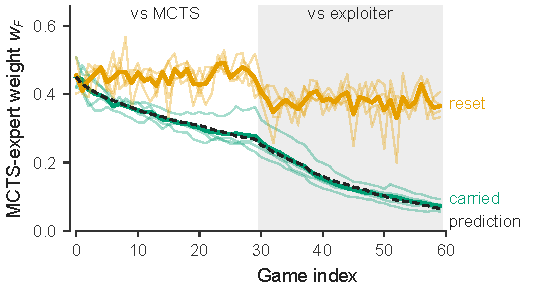
\includegraphics[width=\linewidth]{figures/fig_hedge_half.pdf}
\end{minipage}\hfill
\begin{minipage}[b]{0.46\linewidth}\centering
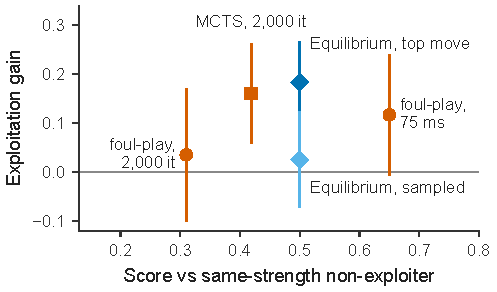
\includegraphics[width=\linewidth]{figures/fig_exploit_half.pdf}
\end{minipage}
\caption{\textbf{Left:} carried Hedge weights move off the MCTS expert, faster once the exploiter starts; reset weights stay near 0.35--0.5. End-of-game MCTS-expert weight $w_F$; thin lines: 4 seeds, thick: mean; shaded: games against the white-box exploiter; dashed: \cref{lem:R3}(b) with per-phase slopes fitted in-sample. \textbf{Right:} only the deterministic bots show a significant LBR exploitation gain. Exploitation gain against the score versus a same-strength non-exploiter (0.5 for the equilibrium bots); bars: 95\% CIs.}
\label{fig:main}
\vspace{-0.6em}
\end{figure}

\subsection{Carrying Hedge weights across games resists an exploiter at no detectable cost}
\label{sec:exp-hedge}
With weights reset each game, Hedge scores 0.560 [0.473, 0.647] against MCTS (100 games) and 0.408 [0.294, 0.522] against a white-box exploiter that knows its mixture $p_t$ (60 games). These come from a different experiment (different seeds and games) than \cref{tab:hedge} (0.471 and 0.388, 120 games); the CIs overlap. We then ran 4 seeds, each with 30 games against MCTS followed by 30 against the exploiter, once with carried and once with reset weights on the same game seeds (\cref{tab:hedge}). Paired on (seed, game), carried minus reset is $+0.062$ [$-0.050$, $+0.175$] against MCTS and $+0.146$ [$+0.039$, $+0.253$] against the exploiter, with CIs over 4 seeds ($t$-distribution, 3 degrees of freedom), so the latter just excludes 0. Carrying weights thus has no detectable cost against MCTS and makes the learner harder to exploit (4 seeds; the CI just excludes 0).

The carried learner runs one long experts problem over the match (\cref{sec:hedge}). Its MCTS-expert weight drifts slowly against MCTS (0.45 to 0.28 over 30 games) and falls faster once the exploiter starts (0.28 to 0.07; \cref{fig:main}, left). \Cref{lem:R3} accounts for this quantitatively. Fitting $G_t$ linearly per phase gives $d_1=0.0133\pm0.0023$ against MCTS and $d_2=0.0291\pm0.0014$ against the exploiter per turn (sd over seeds; $R^2$ between 0.861 and 0.987), and the constant-slope model predicts the logged $w_F$ with maximum error 0.017 over 60 games (RMS 0.006; slopes fitted in-sample; \cref{tab:r3b}). The carried learner meets the exploiter at $w_F\approx0.278$. The implied per-turn surrogate deficit to the equilibrium expert is 0.0040 (carried) against 0.0116 (reset) when facing the exploiter, a ratio of 2.9, and 0.0043 against 0.0051 when facing MCTS, a ratio of 1.2, consistent with the sign and asymmetry of the score differences. Three caveats apply: both experts are rewarded under $\Ahat$, which favours the equilibrium expert by construction; the surrogate explanation holds on average but does not predict per-game outcomes (correlation $-0.17$, $n=120$); and the exploiter's edge does not measurably grow with the MCTS share (coefficient $0.0002\pm0.014$). With the incremental update of \cref{prop:R1}, the carried learner had collapsed onto the equilibrium expert within about 10 games and carried minus reset was $-0.10$ against MCTS, an artefact of that bug.

\begin{table}[h]
\centering\small
\caption{Hedge over \{foul-play, equilibrium sampled\}, carried vs.\ reset weights on the same seeds: 4 seeds $\times$ (30 games against MCTS, then 30 against the white-box exploiter); CIs over seeds ($t_3$).}
\label{tab:hedge}
\begin{tabular}{@{}llcccc@{}}
\toprule
Weights & Opponent & Games & Score & 95\% CI & MCTS-expert weight (end of game, mean) \\
\midrule
Carried & MCTS, 2,000 it & 120 & 0.533 & [0.355, 0.712] & 0.34 \\
Carried & white-box exploiter & 120 & 0.533 & [0.441, 0.625] & 0.14 \\
Reset & MCTS, 2,000 it & 120 & 0.471 & [0.401, 0.541] & 0.45 \\
Reset & white-box exploiter & 120 & 0.388 & [0.308, 0.467] & 0.38 \\
\bottomrule
\end{tabular}
\vspace{-0.6em}
\end{table}

\subsection{Exact endgames point to the leaf as the bottleneck}
\label{sec:exp-end}
We solved small endgames exactly by Shapley iteration under an abstraction with HP buckets, so the resulting values and exploitabilities are exact only for the abstracted game. On every evaluated row \eqref{eq:full} lies above the true exploitability, but it is nearly vacuous: the refined bound divided by the exploitability is 6.9--155 on the 22 rows with exploitability above $10^{-3}$ and a finite bound. The maximum calibrated $\epsv$ reaches 0.8--1.0 nearly everywhere, while $\epss\approx0$. In four representative cases the true exploitability of equilibrium sampled reaches 0.859 payoff units (\cref{tab:endgame}). One exact-equilibrium row has exploitability 0.029 and infinite $\Hbar$ because two reachable states form an endless loop that the abstraction never ends, an instance of the non-termination example of \cref{app:leaf}; the other 11 exact-equilibrium rows are below $2.5\cdot10^{-10}$.

In a preliminary comparison, exact terminals plus $\tanh(h/160)$ cut the exploitability of equilibrium sampled on greattusk vs.\ gholdengo from 0.215 / 0.120 to 0.000 / 0.000 and on gholdengo vs.\ heatran from 0.074 / 0.425 to 0.074 / 0.020, but barely change it on the long, balanced garchomp vs.\ rotomwash (0.338 / 0.602 to 0.306 / 0.601), where the heuristic lacks information rather than calibration. In mid-game play (20 pairs against foul-play at 75\,ms) the current leaf scores $0.375\pm0.15$ and the fixed leaf $0.312\pm0.14$ (20 pairs): no measurable change, as expected since the fix acts on about 12\% of decisions. A learned leaf did not help either (tested only as a depth-1 leaf, without a depth-1 heuristic control): a value net fit to game outcomes (30k MCTS self-play games, 1.1M positions) predicts no better than the heuristic (held-out sign accuracy 0.743 for both on a 2,000-position subsample; 0.726 for the net on the full validation set) and, as a depth-1 leaf, scores 0.235 [0.185, 0.285] against time-matched MCTS, plausibly because the roughly 37 positions of a game share one outcome label.

\subsection{Agent-form solving beats PIMC averaging at equal compute}
\label{sec:exp-hidden}
This is our head-to-head test of PokaiTrainer's agent-form formulation \cite{Yu26}. Under hidden information and equal compute (4 worlds, about 340\,ms per move), the agent-form solve beats the PIMC blend 0.585 [0.540, 0.630] over 400 games. The remaining results for the same comparison are inconclusive: with top-move play it scores 0.540 [0.452, 0.628] (100 games), which crosses 0.5, and against most-likely-set play 0.440 [0.338, 0.542] sampled and 0.525 [0.452, 0.598] top move. Smaller matchups (100 games) are inconclusive, and an agent that sees the true state beats agent-form by about 0.1 (0.600 [0.513, 0.687] with sampled play). Over 46,890 logged decisions the blend's loss never exceeded $4\delta_H$ ($\delta_H$: Hausdorff distance between the worlds' payoff-column sets); the largest loss was 0.098 of that bound. Eight worlds did not beat four (0.495 [0.414, 0.576], 100 games, top-move play). An exploiter that knows the agent-form algorithm and the true state gained 0.00 against sampled and 0.03 against top-move play relative to the true-state agent (40 games each, CIs about $\pm0.13$--$0.16$), which is inconclusive rather than zero.

\subsection{RL best responses give no useful lower bound}
\label{sec:exp-rl}
With 100k training decisions per target, PPO best responses raised their win rate from 0.043 to 0.088 against foul-play (2,000 iterations), from 0.108 to 0.123 against equilibrium sampled and from 0.135 to 0.158 against top move (200 held-out games; CIs about $\pm0.02$--$0.04$). These gains are within noise except possibly against foul-play ($z\approx2.4$ under independence). To test whether the budget was the limit, we trained the best response against foul-play for 8.01M decisions (147,456 games, about $68\times$ the earlier 2.2k games), with the same warm start and held-out seeds. The win rate went 0.060, 0.065, 0.090, 0.100, 0.1225 and 0.125 [0.097, 0.153] at 0, 1.00M, 3.01M, 4.94M, 6.00M and 8.01M decisions, so the lower bound on exploitability stays negative ($-0.375$ [$-0.403$, $-0.347$]). A gray-box variant whose observation also includes foul-play's exact move distribution for the current turn, trained for the same 8.0M decisions, did not do better: 0.055, 0.0925, 0.0975, 0.0825, 0.0825 and 0.075 [0.051, 0.099] at 0, 1M, 3M, 5M, 6M and 8M decisions, ending below the black-box run (single runs; the black-box curve was trained in two parts). Knowing the opponent's policy does not help without a model of the payoffs, which the white-box exploiter has. We attribute the black-box result to the starting point: the self-play pilot net (30M decisions on the 12-species pool) reaches only 0.0625 against MCTS. A useful RL measurement would need a much stronger base policy or a far larger budget, whereas the white-box exploiter certifies 0.250 and 0.090 with no training.

% =====================================================================
\section{Discussion and limitations}
\label{sec:discussion}
No bot dominates: time-matched MCTS is stronger, sampled equilibrium play is less exploitable, and Hedge with carried weights improves robustness without a detectable cost in strength. Four lines of evidence point to the leaf value as the bottleneck: its term in \eqref{eq:headline} does not shrink with compute or depth; time-matched MCTS wins; on exact endgames the calibrated $\epsv$ is near 1 and the bound is loose by 6.9--155$\times$; and a single mis-scored terminal forces a constant calibration (\cref{lem:R6b}). Consequently the upper side of every exploitability bracket is trivial, and our Hedge guarantees hold relative to the surrogate only.

\textbf{Limitations.} The leaf comparison is preliminary, and its mid-game effect rests on 20 pairs. poke-engine's MCTS rounds the iteration count up to a multiple of 1,000, so the 200-iteration MCTS opponent of our PPO pilot actually ran 1,000. Seeded runs are not fully deterministic (1 of 6 local replays diverged at turn 27, and local and cloud runs of one seed differed), so pairing is approximate. The white-box exploiter's pruning affects only the sampled target, and it has no same-depth non-modelling control. Moves count as revealed when chosen, items and abilities are never inferred, the team generator is approximate, and 2--30\% of games reach the 300-turn cap (up to 40\% for LBR in the white-box runs) and count as draws. Most hidden-information matchups have 100 games (CI about $\pm0.09$) and the LBR runs 30 pairs. Our leaves ignore beliefs, so concealment has no value in our model (\cref{asm:world}). We did not deploy on Showdown, and the behavioural opponent memory from our proposal was not built.

% =====================================================================
\section{Conclusion}
\label{sec:conclusion}
Per-turn equilibrium play in Random Battles has a clean error budget whose dominant term, the leaf error, does not shrink with compute, and our experiments agree: equilibrium play loses to time-matched MCTS, sampled equilibrium play is more robust than deterministic play but still has a certified exploitability of at least 0.090 in score (win-rate) units, and Hedge with carried weights is harder to exploit at no detectable cost. Exact terminals fix the easy endgames but not the balanced one. The most promising next steps are a better leaf, such as a value net trained on low-variance absolute targets with exact terminals, and a same-depth control for the white-box exploiter.

% =====================================================================
\begin{multicols}{2}
\begin{thebibliography}{99}\scriptsize
\setlength{\itemsep}{0pt}\setlength{\parsep}{0pt}\setlength{\parskip}{0pt}
\bibitem{Yu26} M.~Yu. PokaiTrainer: Scaling equilibrium search to competitive Pok\'emon VGC. arXiv:2608.29197, 2026.
\bibitem{foulplay} P.~Mariglia. Foul Play: a competitive Pok\'emon Showdown battle bot. \url{https://github.com/pmariglia/foul-play}; engine \url{https://github.com/pmariglia/poke-engine}, 2024.
\bibitem{jaxcalibur} Anonymous (Smogon user jaxcalibur\_author). Jaxcalibur: how Jaxcalibur works. \url{https://jaxcalibur.github.io/} (accessed 2026-11-15). Self-reported, not peer reviewed, code and weights not released.
\bibitem{Shapley53} L.~S.~Shapley. Stochastic games. PNAS 39(10):1095--1100, 1953.
\bibitem{Fra98} I.~Frank, D.~Basin. Search in games with incomplete information: a case study using Bridge card play. Artificial Intelligence, 1998.
\bibitem{Lon10} J.~Long, N.~R.~Sturtevant, M.~Buro, T.~Furtak. Understanding the success of perfect information Monte Carlo sampling in game tree search. AAAI, 2010.
\bibitem{CFRD} N.~Burch, M.~Johanson, M.~Bowling. Solving imperfect information games using decomposition (CFR-D). AAAI, pp.~602--608, 2014; arXiv:1303.4441.
\bibitem{Mor17} M.~Morav\v{c}\'{\i}k et~al. DeepStack: expert-level artificial intelligence in heads-up no-limit poker. Science, 2017.
\bibitem{Bro20} N.~Brown, A.~Bakhtin, A.~Lerer, Q.~Gong. Combining deep reinforcement learning and search for imperfect-information games. NeurIPS, 2020.
\bibitem{Tam14} O.~Tammelin. Solving large imperfect information games using CFR+. arXiv:1407.5042, 2014.
\bibitem{Tammelin15} O.~Tammelin, N.~Burch, M.~Johanson, M.~Bowling. Solving heads-up limit Texas hold'em. IJCAI, 2015.
\bibitem{BMS19} N.~Burch, M.~Morav\v{c}\'{\i}k, M.~Schmid. Revisiting CFR+ and alternating updates. JAIR 64:429--443, 2019; arXiv:1810.11542.
\bibitem{BLM13} S.~Boucheron, G.~Lugosi, P.~Massart. Concentration Inequalities: A Nonasymptotic Theory of Independence. Oxford University Press, 2013.
\bibitem{Gan15} S. Ganzfried, T. Sandholm. Safe opponent exploitation. ACM Trans. Economics and Computation, 2015.
\bibitem{Hannan57} J.~Hannan. Approximation to Bayes risk in repeated play. In M.~Dresher, A.~W.~Tucker, P.~Wolfe, eds., Contributions to the Theory of Games III, Annals of Mathematics Studies 39, pp.~97--139. Princeton University Press, 1957.
\bibitem{LW94} N.~Littlestone, M.~K.~Warmuth. The weighted majority algorithm. Information and Computation 108(2):212--261, 1994.
\bibitem{CS535L6} CS535 Algorithmic Game Theory, Lecture 6: Learning in Games and Playing Against Nature; Lecture 7: No-Regret Dynamics in Games, 2026.
\bibitem{FS97} Y.~Freund, R.~E.~Schapire. A decision-theoretic generalization of on-line learning and an application to boosting. JCSS 55(1):119--139, 1997.
\bibitem{HW98} M.~Herbster, M.~K.~Warmuth. Tracking the best expert. Machine Learning 32(2):151--178, 1998.
\bibitem{CBL06} N.~Cesa-Bianchi, G.~Lugosi. Prediction, Learning, and Games. Cambridge University Press, 2006.
\bibitem{Aro12b} R.~Arora, O.~Dekel, A.~Tewari. Online bandit learning against an adaptive adversary: from regret to policy regret. ICML, 2012.
\bibitem{OP18} F.~Orabona, D.~P\'al. Scale-free online learning. Theoretical Computer Science 716:50--69, 2018; arXiv:1601.01974.
\bibitem{Tim20} F.~Timbers et~al. Approximate exploitability: learning a best response in large games. arXiv:2004.09677, 2020.
\bibitem{Everett57} H.~Everett. Recursive games. Contributions to the Theory of Games III, Ann.\ Math.\ Studies 39, 1957.
\bibitem{DS65} L.~E.~Dubins, L.~J.~Savage. How to Gamble If You Must: Inequalities for Stochastic Processes. McGraw-Hill, 1965.
\bibitem{MS96} A.~P.~Maitra, W.~D.~Sudderth. Discrete Gambling and Stochastic Games. Springer, 1996.
% --- no-regret vs RL framing; entries from lit/noregret_vs_rl.md ---
\bibitem{Rud25} M.~Rudolph, N.~Lichtle, S.~Mohammadpour, A.~Bayen, J.~Z.~Kolter, et~al. Reevaluating policy gradient methods for imperfect-information games. arXiv:2502.08938, 2025.
\bibitem{Sok23} S.~Sokota, R.~D'Orazio, J.~Z.~Kolter, N.~Loizou, M.~Lanctot, I.~Mitliagkas, N.~Brown, C.~Kroer. A unified approach to reinforcement learning, quantal response equilibria, and two-player zero-sum games. ICLR, 2023; arXiv:2206.05825. % CHECK VENUE
\bibitem{Per22} J.~Perolat, B.~de~Vylder, D.~Hennes, et~al. Mastering the game of Stratego with model-free multiagent reinforcement learning. Science 378(6623), 2022; doi:10.1126/science.add4679.
\bibitem{Sch23} M.~Schmid et~al. Student of Games: a unified learning algorithm for both perfect and imperfect information games. Science Advances, 2023; arXiv:2112.03178. % CHECK VENUE (and full title)
\bibitem{Lis13} V.~Lis\'y, V.~Kova\v{r}\'{\i}k, M.~Lanctot, B.~Bo\v{s}ansk\'y. Convergence of Monte Carlo tree search in simultaneous move games. NeurIPS, pp.~2112--2120, 2013; arXiv:1310.8613.
\bibitem{Lis17} V.~Lis\'y, M.~Bowling. Equilibrium approximation quality of current no-limit poker bots. AAAI-17 Workshop on Computer Poker and Imperfect Information Games; arXiv:1612.07547, 2016. % CHECK VENUE
\bibitem{Lan17} M.~Lanctot, V.~Zambaldi, A.~Gruslys, et~al. A unified game-theoretic approach to multiagent reinforcement learning. NeurIPS, 2017; arXiv:1711.00832. % CHECK VENUE
\bibitem{Wang23} T.~T.~Wang, A.~Gleave, T.~Tseng, K.~Pelrine, N.~Belrose, J.~Miller, et~al. Adversarial policies beat superhuman Go AIs. ICML, 2023; arXiv:2211.00241. % CHECK VENUE (and initials)
\bibitem{Aga21} A.~Agarwal, S.~M.~Kakade, J.~D.~Lee, G.~Mahajan. On the theory of policy gradient methods: optimality, approximation, and distribution shift. JMLR 22(98), 2021; arXiv:1908.00261. % CHECK VENUE
\bibitem{Tom22} M.~Tomar, L.~Shani, Y.~Efroni, M.~Ghavamzadeh. Mirror descent policy optimization. ICLR, 2022; arXiv:2005.09814. % CHECK VENUE
\bibitem{Sha20} L.~Shani, Y.~Efroni, S.~Mannor. Adaptive trust region policy optimization: global convergence and faster rates for regularized MDPs. AAAI, 2020; arXiv:1909.02769. % CHECK VENUE
\bibitem{Pol19} Y.~Abbasi-Yadkori, P.~Bartlett, K.~Bhatia, N.~Lazic, C.~Szepesv\'ari, G.~Weisz. POLITEX: regret bounds for policy iteration using expert prediction. ICML, PMLR 97:3692--3702, 2019.
\bibitem{Ross11} S.~Ross, G.~J.~Gordon, J.~A.~Bagnell. A reduction of imitation learning and structured prediction to no-regret online learning. AISTATS, 2011; arXiv:1011.0686. % CHECK VENUE
\bibitem{Mun07} R.~Munos. Performance bounds in $L_p$-norm for approximate value iteration. SIAM J.\ Control Optim.\ 46(2), 2007; doi:10.1137/040614384.
\bibitem{Sch15} B.~Scherrer, M.~Ghavamzadeh, V.~Gabillon, B.~Lesner, M.~Geist. Approximate modified policy iteration and its application to the game of Tetris. JMLR 16, 2015; arXiv:1205.3054. % CHECK VENUE
\bibitem{Per15} J.~P\'erolat, B.~Scherrer, B.~Piot, O.~Pietquin. Approximate dynamic programming for two-player zero-sum Markov games. ICML, PMLR 37:1321--1329, 2015.
\bibitem{Tian21} Y.~Tian, Y.~Wang, T.~Yu, S.~Sra. Online learning in unknown Markov games. ICML, 2021; arXiv:2010.15020. % CHECK VENUE
\bibitem{Liu22} Q.~Liu, Y.~Wang, C.~Jin. Learning Markov games with adversarial opponents: efficient algorithms and fundamental limits. ICML, 2022; arXiv:2203.06803. % CHECK VENUE
\bibitem{KS02} M.~Kearns, S.~Singh. Near-optimal reinforcement learning in polynomial time. Machine Learning 49, 2002; doi:10.1023/A:1017984413808.
\end{thebibliography}
\end{multicols}

% =====================================================================
\appendix
\section{Proof sketches}
\label{app:proofs}

\textbf{\Cref{lem:one}.} For all mixed $x,y$, $|x^\top(A-B)y|\le\varepsilon$, hence $|\val A-\val B|\le\varepsilon$. Then $\min_yx^\top Ay\ge\min_yx^\top By-\varepsilon\ge\val B-\epss-\varepsilon\ge\val A-\epss-2\varepsilon$. Tightness: $A=(0,-2\varepsilon)^\top$, $B=(-\varepsilon,-\varepsilon)^\top$ and $x=e_2$.

\textbf{\Cref{thm:full}.} Fix $\sigma$. On live histories define $D_t(h)=\delta(t,s_t)+\E[D_{t+1}\mid h]$, and $D=0$ otherwise. Suppose $W_{t+1}\ge\Vstar_{t+1}-D_{t+1}$ on every child. With $x$ the agent's stage strategy and $y=\sigma(h)$, $W_t(h)\ge x^\top\Qstar_t(s)y-(D_t-\delta)$, and \cref{lem:one} with $A=\Qstar_t(s)$, $B=\Qhat_t(s)$ gives $x^\top\Qstar_t(s)y\ge\Vstar_t(s)-\delta$, which closes the induction. Since the induction runs over histories, the opponent may condition on past realised actions. Taking $\sigma=\sigma^\star$ and $\delta\le\epss+2\epsv$ gives \eqref{eq:full}. \emph{Tightness of $\Hbar$.} Take states $s_c$ and terminals $z_c$ with $u(z_c)=-c\delta$; the agent picks $g$ or $b$, the opponent ``end'' or ``cont'', and $b$ increments $c$. Then $\Vstar_0=0$ and $x=e_b$ is $\delta$-optimal; ``end at once'' is minimax-optimal with length 1, but ``cont always'' yields $-H\delta$, so $\expl=H\delta$.

\textbf{\Cref{prop:rm}.} The RM$^+$ accumulator satisfies $\lVert Q_T\rVert_2\le\Delta\sqrt{nT}$~\cite{Tam14}. With one virtual row update, the linearly weighted gap decomposes into both players' weighted regrets plus a cross term $\sum_tt\,[u(x_t,y_t)-u(x_t,y_{t-1})]$ from the alternation, which is $\le0$ term by term because an RM$^+$ update never lowers the updating player's utility against the vector that produced it (\cite{BMS19}, Thm~5). This gives $\mathrm{gap}\le2\Delta(\sqrt{n(T+1)}+\sqrt{mT})/(T+1)$.

\textbf{\Cref{prop:K}.} The agent-form objective is $\frac\Delta2$-Lipschitz in $\ell_1$. Combine a $(3/\varepsilon)^n$ net of the simplex at $\varepsilon=K^{-1/2}$, Hoeffding's inequality and the sub-Gaussian maximal inequality~\cite{BLM13}.

\textbf{\Cref{thm:C}.} Since the sampled worlds are fresh and unobserved, the opponent faces the expected mixture $\tilde x$. The agent-form objective $f_b$ is concave, so $f_b(\tilde x)\ge v(b)-(\epss+2\epsv+\text{sampling})$. Two applications of $|f_b-f_p|\le\Delta\TV(b,p)$ convert this to the true posterior $p$, giving the $4\TV$ term on $[-1,1]$. The revealed stage payoff and the true belief-dependent payoff differ by at most $\etaNL$, and the value is convex in the belief, so the induction of \cref{thm:full} goes through with the two extra terms.

\textbf{\Cref{lem:R2}.} Use the potential $\Phi_t(\beta)=\beta^{-1}\ln(\frac1k\sum_ie^{\beta L_{t,i}})$. Each step costs at most $w_t\cdot r_t+\beta_t/8$ by Hoeffding's lemma, and $\Phi_t$ is nondecreasing in $\beta$, so decreasing step sizes only help; telescope. Substituting $\beta_t=\eta_{t-1}$ gives the stated constant.

\textbf{\Cref{prop:E1}.} Normalising each turn by $\range\Ahat_t$ instead admits a raw-unit deficit of $S/3$ against an opponent that switches columns with the stakes. The reward is affine in the expert's strategy, so the learner's reward is $w_t\cdot r_t$ when nothing is clipped. Compare with $e=N$, whose surrogate payoff is at least $\val\Ahat_t-\epss$ whatever $b_t$ is, and multiply the regret bound by $\Dbar$. \emph{Across games.} If $\lVert a\Ahat_t+c-\Qstar_t\rVert_\infty\le\epsv^{\rm glob}$ with $a>0$ at every learner turn, then by affine invariance of RM$^+$, \cref{lem:one} per turn, \cref{lem:R2} and $\E\sqrt S\le\sqrt{J\Hbar_\sigma}$, the average over $J$ games of $\Vstar_0-\E_\sigma[u_g]$ is at most $\Hbar_\sigma(a\epss+2\epsv^{\rm glob})+400a\big(3\sqrt{\Hbar_\sigma\ln k/(8J)}+\frac1J\sqrt{\ln k/8}\big)+\E_\sigma[C_S]/J$, where $C_S=\sum_{t\le S}a(\range\Ahat_t-400)^+$ is the clipping loss (the clipping term is nonzero on the roughly 6\% of learner turns with $\range\Ahat_t>400$; a reward is actually clipped on about 0.5\%) and $\Hbar_\sigma$ is the mean game length against $\sigma$. The calibration must be global: exact per-turn slopes alternating between $1/200$ and $0.01/200$ lose 0.248 per turn.

\textbf{\Cref{prop:R1}.} Write $s_n=\sum_{j\le n}j^{-1/2}$, so $2\sqrt{n+1}-2\le s_n\le2\sqrt n$. After phase 1 the log-weight gap is $\Lambda_t=c(2s_{T_1}-s_{t-1})$. For $t\le4\theta^2T_1$ it is at least $2c(2(1-\theta)\sqrt{T_1}-2)\to\infty$, so the learner misses phase-2 reward until about $4\alpha T$; for $t\ge4T_1/\theta^2$ it tends to $-\infty$. Letting $\theta\uparrow1$ gives matching limits, whereas FTRL's leader switches at $2\alpha T$.

\textbf{\Cref{lem:R3}.} (a) is the FTRL weight formula for $k=2$; (b) substitutes $G_t=dt$ and $\eta_t=\sqrt{8\ln2/t}$; (c) expands $p_t=w_Nq_N+w_Fq_F$ and uses the definition of the rewards.

\textbf{\Cref{prop:R5}.} (a) is Hoeffding's inequality for each fixed exploiter and a union bound over $m_X$; (b) follows by adding and subtracting $s(\pi,\beta)$ and using $s(\pi,X)\ge v^\star-\expl(\pi)$ and $s(\pi,\beta)\le v^\star+\expl(\beta)$.

\textbf{\Cref{lem:R6b}.} For fixed $a$ the best $c$ centres $aM_i-Q_i$, giving $\frac12\max_{i,j}[(Q_i-Q_j)-a(M_i-M_j)]$, which is convex and piecewise linear in $a$; $a=0$ is optimal iff its right derivative at 0 is nonnegative, i.e.\ iff some pair $i\in\argmax Q$, $j\in\argmin Q$ has $M_i\le M_j$.

\textbf{\Cref{prop:visits} and links to RL.} For any potential $\Phi$ on histories with $\Phi=u$ at terminals, $\Phi_0-V(\pi,\sigma)=\E_{\pi,\sigma}[\sum_{t<\tau}(\Phi_t-x_t^\top Q[\Phi]_ty_t)]$, because simultaneous moves make $a_t$ and $b_t$ independent given the history. With $\Phi=\Vstar$ this gives \cref{thm:full} as an identity. At one MCTS node, summing both sides' regrets cancels the realised joint terms, so the Nash gap of the visit shares equals $(\Reg^1_N+\Reg^2_N)/N$; on $\Ahat=[[.5,.9],[.1,.5]]$, whose first row is dominant, decoupled UCB1 with deterministic rewards and first-index tie-breaking plays in lockstep and keeps a gap of $0.4$ for every even $N$. With $\Phi=V^{\pi,\sigma_k}$ in the opponent's MDP the identity is the performance-difference lemma, and averaging natural-policy-gradient iterates gives per-state Hedge regret weighted by the best response's state distribution, whose total mass is $\Hbar$.

\textbf{Formalisation.} The one-step lemma (\cref{lem:one}) and the backward-induction step of \cref{thm:full} were formalised in Lean~4.

\section{Secondary theory}
\label{app:secondary}
\subsection{Hidden information: sampled worlds and the general case}
\label{sec:general}
\begin{proposition}[sampled worlds]\label{prop:K}
Solving $K\ge9$ sampled worlds instead of the exact belief adds, in expectation, at most $2\Delta\sqrt{2(n\log K+\log2)/K}\approx4\sqrt{2n\log K/K}$ to the per-turn budget.
\end{proposition}
Drop \cref{asm:nonrev,asm:world}. Let $\etaNL(t)$ be the largest value, over positions and beliefs at turn $t+1$, of revealing the opponent's type to both sides, and let $\TV$ be the total-variation distance between the true posterior under the opponent's actual strategy and our hard-evidence belief.
\begin{theorem}[hidden information]\label{thm:C}
Under \cref{asm:prior}, for every history-dependent opponent that knows its own type,
$\expl(\pi)\le\Hbar\big(8\sqrt{n/T}+2\epsv+4\sqrt{2n\log K/K}+\etaNL+4\,\TV\big)$. Here $\etaNL=0$ under \cref{asm:world} and $\TV=0$ under \cref{asm:nonrev}.
\end{theorem}
Both extra terms are necessary: in a three-type, two-turn example where the agent solves the exact belief game (solver, leaf and sampling terms 0), $\expl=1$ while $\sum_t\etaNL(t)=3/7$, so without $\TV$ the bound fails against a revealing opponent. Belief-dependent leaves~\cite{CFRD,Mor17,Bro20} remove $\etaNL$; ours do not.

\subsection{How loose the constants are}
\label{app:const}
On 35 real stage matrices the measured RM$^+$ gap is at most 0.04 of the bound of \cref{prop:rm} and falls as $\approx T^{-1.3}$, and the sampling bound of \cref{prop:K} becomes informative only once $K/\log K\gtrsim2n$, which $K=4$ does not reach.

\subsection{Leaf diagnostics}
\label{app:leaf}
\begin{lemma}[inversions force a constant calibration]\label{lem:R6b}
$\epsv^{\rm cal}\ge\frac12\max\{\Qstar_i-\Qstar_j:\Qhat_i\le\Qhat_j\}$ over cells $i,j$, and $a=0$ is an optimal calibration if and only if some cell in $\argmax\Qstar$ is scored at or below some cell in $\argmin\Qstar$. If terminal children are scored exactly, cells whose children are all terminal are exact.
\end{lemma}
\textbf{Non-termination.} In a one-state game where one action ends the game at $0.3$, another ends it at $0.8$ if the opponent stops and loops otherwise, and endless play pays 0, the stage-maximin agent ``always continue'' has zero stage budget yet exploitability $0.3$; with a turn cap, \cref{thm:full} holds with equality and charges the whole $0.3$ to the last turn. This is the Everett and Dubins--Savage phenomenon~\cite{Everett57,DS65,MS96}; the minimal example is ours.

\subsection{Anytime updates and weight dynamics}
\begin{proposition}[incremental anytime updates have linear regret]\label{prop:R1}
Let $\lambda_{t+1}=\lambda_t+(c/\sqrt t)\,r_t$ and $w_t\propto e^{\lambda_t}$. With rewards $e_1$ for the first $\lfloor\alpha T\rfloor$ turns and $e_2$ afterwards, $\lim_{T\to\infty}\Reg_T/T=\kappa(\alpha)=\min(2\alpha,1-2\alpha)^+$, independently of $c$ and $k$; in particular $\kappa(0.3)=0.40$, and the maximum is $\kappa(1/4)=1/2$.
\end{proposition}
Orabona and P\'al~\cite{OP18} prove $\Reg_T\ge T/6$ for this update on the same kind of sequence with phases $T/3$ and $2T/3$; the exact limit for every $\alpha$ (for instance $\kappa(1/3)=1/3$) and its independence of $c$ and $k$ are new. Our first implementation used this update; on a 30/70 phase switch it had regret $0.4001\,T$ at $T=10^4$, against 1.46 for FTRL at $T=10^3$ to $10^5$. All Hedge results use FTRL.

\begin{lemma}[weight dynamics, $k=2$]\label{lem:R3}
Let $G_t=L_{t,N}-L_{t,F}$ and $d_t=r_{t,N}-r_{t,F}$. Under FTRL, (a) $\ln(w_N/w_F)=\eta_tG_t$; (b) if $d_j\equiv d$, then $w_F=\lgs(-d\sqrt{8\ln2}\,\sqrt t)$, with $\lgs$ the logistic function; (c) $p_t\cdot\Ahat_t[:,b_t]=q_{N,t}\cdot\Ahat_t[:,b_t]-400\,w_{F,t}\tilde d_t$, where $\tilde d_t=d_t$ when no reward is clipped.
\end{lemma}
The MCTS share thus decays with log-odds proportional to $\sqrt t$, and the learner's per-turn surrogate deficit to the equilibrium expert is proportional to that share. A reset learner restarts at $t=1$ every game, so by (b) its $w_F$ falls only to about $0.40$ by the end of a typical game, whereas a carried learner keeps accumulating evidence.

\subsection{Measuring exploitability}
\label{sec:measure}
Exact exploitability is computable only on small endgames, so we bound it from below with explicit exploiters.
\begin{proposition}[lower bounds from exploiters]\label{prop:R5}
Let exploiters $X_1,\dots,X_{m_X}$ be legal strategies fixed before the seeds are drawn, each evaluated on $\nu$ independent seat-swapped pairs with mean score $\bar Z_j$. (a) With probability at least $1-\vartheta$, $\expl(\pi)\ge\max_j\bar Z_j-v^\star-\sqrt{\ln(m_X/\vartheta)/(2\nu)}$ in score units; re-evaluating the selected exploiter on fresh pairs removes the $\ln m_X$. (b) For a non-exploiting baseline $\beta$ of similar strength, the exploitation gain $\gain=s(\pi,\beta)-s(\pi,X)$ satisfies $\gain\le\expl(\pi)+\expl(\beta)$; it is a lower bound on $\expl(\pi)$ only if $s(\pi,\beta)\le v^\star$, and then it never exceeds $v^\star-s(\pi,X)$.
\end{proposition}
Without the selection correction the best of several zero-edge exploiters is biased upward, by $+0.067$ for $m_X=3$ and $+0.121$ for $m_X=10$ at $\nu=20$. The gain measures how much of an exploiter's success comes from modelling the target, and reads as exploitability only when $\expl(\beta)\ll\gain$. The upper side of the bracket is \cref{thm:full}; with the leaf errors we measure, it is the trivial $\frac12$.

\subsection{RL best responses}
The telescoping identity behind \cref{thm:full} also shows that an RL best response with natural-policy-gradient updates is per-state Hedge in the opponent's induced MDP~\cite{Aga21}, with the same horizon factor $\Hbar$ and a critic term that grows with the mismatch between the learner's and the best response's state distributions (\cref{app:proofs}).

\section{Additional tables}
\label{app:tables}
\begin{table}[h]
\centering\small
\begin{minipage}[t]{0.49\linewidth}\centering
\captionof{table}{True exploitability (payoff units) of equilibrium sampled on abstracted endgames, seat 1 / seat 2.}
\label{tab:endgame}
\footnotesize\setlength{\tabcolsep}{2.5pt}\begin{tabular}{@{}lccc@{}}
\toprule
Case (100\% HP) & Expl. & $\Hbar$ & Refined bound \\
\midrule
garchomp vs.\ rotomwash & 0.338 / 0.602 & 3.2 / 3.0 & 4.5 / 4.6 \\
greattusk vs.\ gholdengo & 0.215 / 0.120 & 1.1 / 1.0 & 2.0 / 2.0 \\
gholdengo vs.\ heatran & 0.074 / 0.425 & 2.0 / 31.4 & 1.6 / 16.4 \\
greattusk vs.\ rotomwash & 0.190 / 0.859 & 2.6 / 6.7 & 2.9 / 10.8 \\
\bottomrule
\end{tabular}
\end{minipage}\hfill
\begin{minipage}[t]{0.48\linewidth}\centering\setlength{\tabcolsep}{2.5pt}
\captionof{table}{Logged vs.\ predicted MCTS-expert weight $w_F$ (carried weights, mean over 4 seeds; constant-slope model of \cref{lem:R3}(b)).}
\label{tab:r3b}
\begin{tabular}{@{}lccccccc@{}}
\toprule
Game & 0 & 9 & 19 & 29 & 39 & 49 & 59 \\
\midrule
Turns $t$ & 45 & 332 & 640 & 1028 & 1462 & 1934 & 2505 \\
Logged & 0.452 & 0.359 & 0.306 & 0.278 & 0.162 & 0.106 & 0.072 \\
Predicted & 0.450 & 0.362 & 0.312 & 0.268 & 0.166 & 0.106 & 0.065 \\
\bottomrule
\end{tabular}
\end{minipage}
\end{table}

\end{document}
